\documentclass[tikz,border=8pt]{standalone}
\usepackage{xcolor}
\usepackage{tikz}
\usetikzlibrary{positioning,fit,backgrounds,arrows.meta}

% Tutorial palette colors
\definecolor{sqfill}{HTML}{ccccff}    % passive Sq: light lavender
\definecolor{sqstroke}{HTML}{000099}  % passive Sq stroke: dark navy
\definecolor{ifill}{HTML}{7373ff}     % interface Sq: bright blue-violet
\definecolor{istroke}{HTML}{0000cc}   % interface Sq stroke: bright blue
\definecolor{newfill}{HTML}{ffbf80}   % new node: light orange
\definecolor{newstroke}{HTML}{cc6600} % new node stroke: burnt orange
\definecolor{boxfill}{HTML}{f5f5f5}   % ACSet bounding box fill
\definecolor{boxstroke}{HTML}{a6a6a6} % ACSet bounding box stroke

\tikzset{
  sqI/.style={circle, fill=ifill, draw=istroke, line width=1pt,
              minimum size=18pt, inner sep=0pt, font=\small},
  newnode/.style={circle, fill=newfill, draw=newstroke, line width=1pt,
                  minimum size=18pt, inner sep=0pt, font=\small},
  acsbox/.style={draw=boxstroke, fill=boxfill, rounded corners=4pt,
                 inner sep=8pt},
  morpharrow/.style={-{Latex[length=5pt,width=3.5pt]}, thick},
  spanarrow/.style={-{Latex[length=5pt,width=3.5pt]}, thick,
                    shorten <=4pt, shorten >=4pt}
}

% mark_x span: L <-l- K -r-> R
% L = K = one bare Sq (identity left leg)
% R = Sq + X connected by xsq
\begin{document}
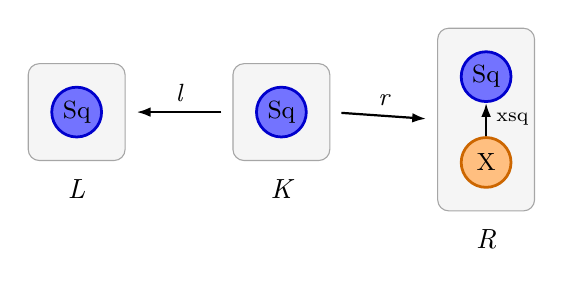
\begin{tikzpicture}

  % --- L (left ACSet): one interface Sq ---
  \node[sqI] (L-sq) at (0, 0) {Sq};
  \begin{pgfonlayer}{background}
    \node[acsbox, fit=(L-sq)] (Lbox) {};
  \end{pgfonlayer}
  \node[below=3pt of Lbox, font=\itshape] {L};

  % --- K (center ACSet): one interface Sq ---
  \node[sqI] (K-sq) at (2.6, 0) {Sq};
  \begin{pgfonlayer}{background}
    \node[acsbox, fit=(K-sq)] (Kbox) {};
  \end{pgfonlayer}
  \node[below=3pt of Kbox, font=\itshape] {K};

  % --- R (right ACSet): interface Sq + new X ---
  \node[sqI]    (R-sq) at (5.2,  0.45) {Sq};
  \node[newnode, below=12pt of R-sq] (R-x) {X};
  \draw[morpharrow] (R-x) -- node[right, font=\scriptsize]{xsq} (R-sq);
  \begin{pgfonlayer}{background}
    \node[acsbox, fit=(R-sq)(R-x)] (Rbox) {};
  \end{pgfonlayer}
  \node[below=3pt of Rbox, font=\itshape] {R};

  % --- Span arrows ---
  % l : K -> L  (left leg, identity)
  \draw[spanarrow] (Kbox.west) -- node[above, font=\small\itshape]{l} (Lbox.east);
  % r : K -> R  (right leg)
  \draw[spanarrow] (Kbox.east) -- node[above, font=\small\itshape]{r} (Rbox.west);

\end{tikzpicture}
\end{document}
